\documentclass[a4paper,11pt]{ujreport}
%%【PostScript, JPEG, PNG等の画像の貼り込み】
%% 利用するパッケージを選んでコメントアウトしてください.
\usepackage{graphicx} % for 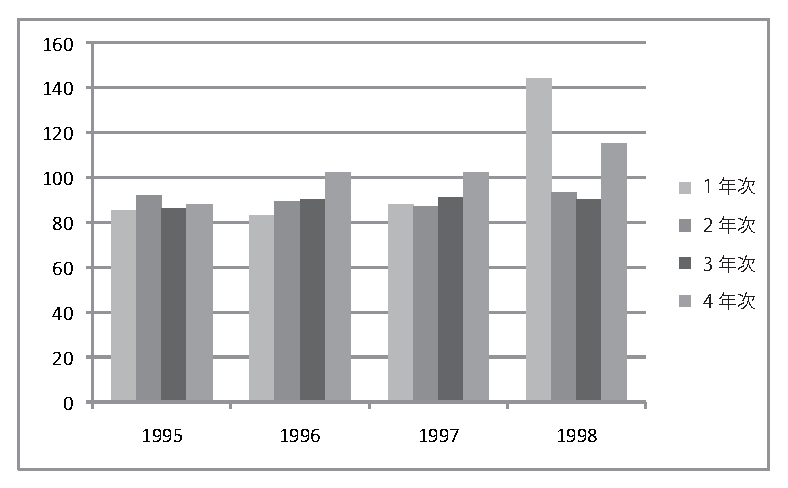
\includegraphics[width=3cm]{sample.eps}
\usepackage{epsfig} % for 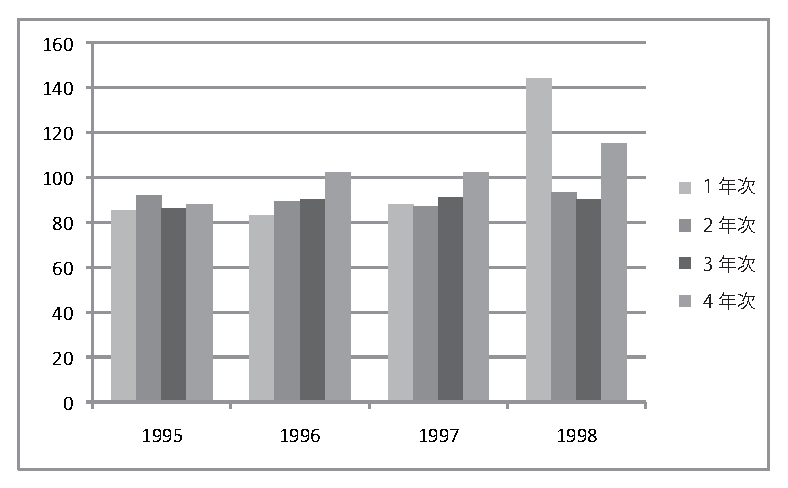
\psfig{file=sample.eps,width=3cm}
%\usepackage{epsf} % for \epsfile{file=sample.eps,scale=0.6}
%\usepackage{epsbox} % for \epsfile{file=sample.eps,scale=0.6}
\usepackage{/Users/takagihayata/workspace/materialize-mongodb/paper/mast/class/mediabb} % for pdf

\usepackage{times} % use Times Font instead of Computer Modern
% \usepackage{listings} % for soursecode
% \usepackage{plistings} % for soursecode
\usepackage{/Users/takagihayata/workspace/materialize-mongodb/paper/mast/class/docmute} % texファイル分割用

\setcounter{tocdepth}{3}
\setcounter{page}{-1}

\setlength{\oddsidemargin}{0.1in}
\setlength{\evensidemargin}{0.1in}
\setlength{\topmargin}{0in}
\setlength{\textwidth}{6in}
%\setlength{\textheight}{10.1in}
\setlength{\parskip}{0em}
\setlength{\topsep}{0em}

%\newcommand{\zu}[1]{{\gt \bf 図\ref{#1}}}

%% タイトル生成用パッケージ(重要)
\usepackage{/Users/takagihayata/workspace/materialize-mongodb/paper/mast/class/mast-jp-sjis}

%% タイトル
%% 【注意】タイトルの最後に\\ を入れるとエラーになります
\title{NoSQL型データベースシステムでの実体化ビュー選択に関する研究}
%% 著者
\author{髙木 颯汰}
%% 指導教員
\advisor{古瀬 一隆 陳 漢雄}

%% 年月 (提出年月)
%% 年月は必要に応じて書き替えてください.
\majorfield{ } \yearandmonth{2019年 1月}


\addtocounter{page}{2} %単体でコンパイルした際の調整用
\begin{document}

\chapter{提案手法}
\label{chap:ProposedAlgorithm}
\section{ドキュメント指向型データベースにおける実体化について}
ドキュメント指向型データベースの特徴として埋め込み(embed)がある.従来のRDBでは複数の表による1対多や多対多の関係を表す際に,参照先のプライマリーキーのみを保存してSELECTされる際に結合処理を行う.それに対してドキュメント指向型データベースでは参照先の実データを参照元に埋め込むことができ,これによって結合処理を省くことができる.埋め込み先が複数の場合には更新処理が増加し,従来の参照型に比べてデータアクセスの柔軟性が損なわれるというデメリットがある\cite{Sky株式会社201212}.図\ref{figure:Reference}はドキュメント指向型データベースの参照型を,図\ref{figure:Embed}は図\ref{figure:Reference}のデータを埋込型で表した図である.
また.図\ref{figure:Reference}と図\ref{figure:Embed}のドキュメントを得るためのクエリを表\ref{table:MongoReferenceEmbedFind}に示す.idが123456のドキュメントを更新するクエリを表\ref{table:MongoReferenceEmbedUpdate}に示す.なお,表\ref{table:MongoReferenceEmbedUpdate}の埋込型に関しては,埋め込まれているコレクション全てに対してクエリを実行する必要がある.
\begin{figure}[htbp]
	\begin{center}
		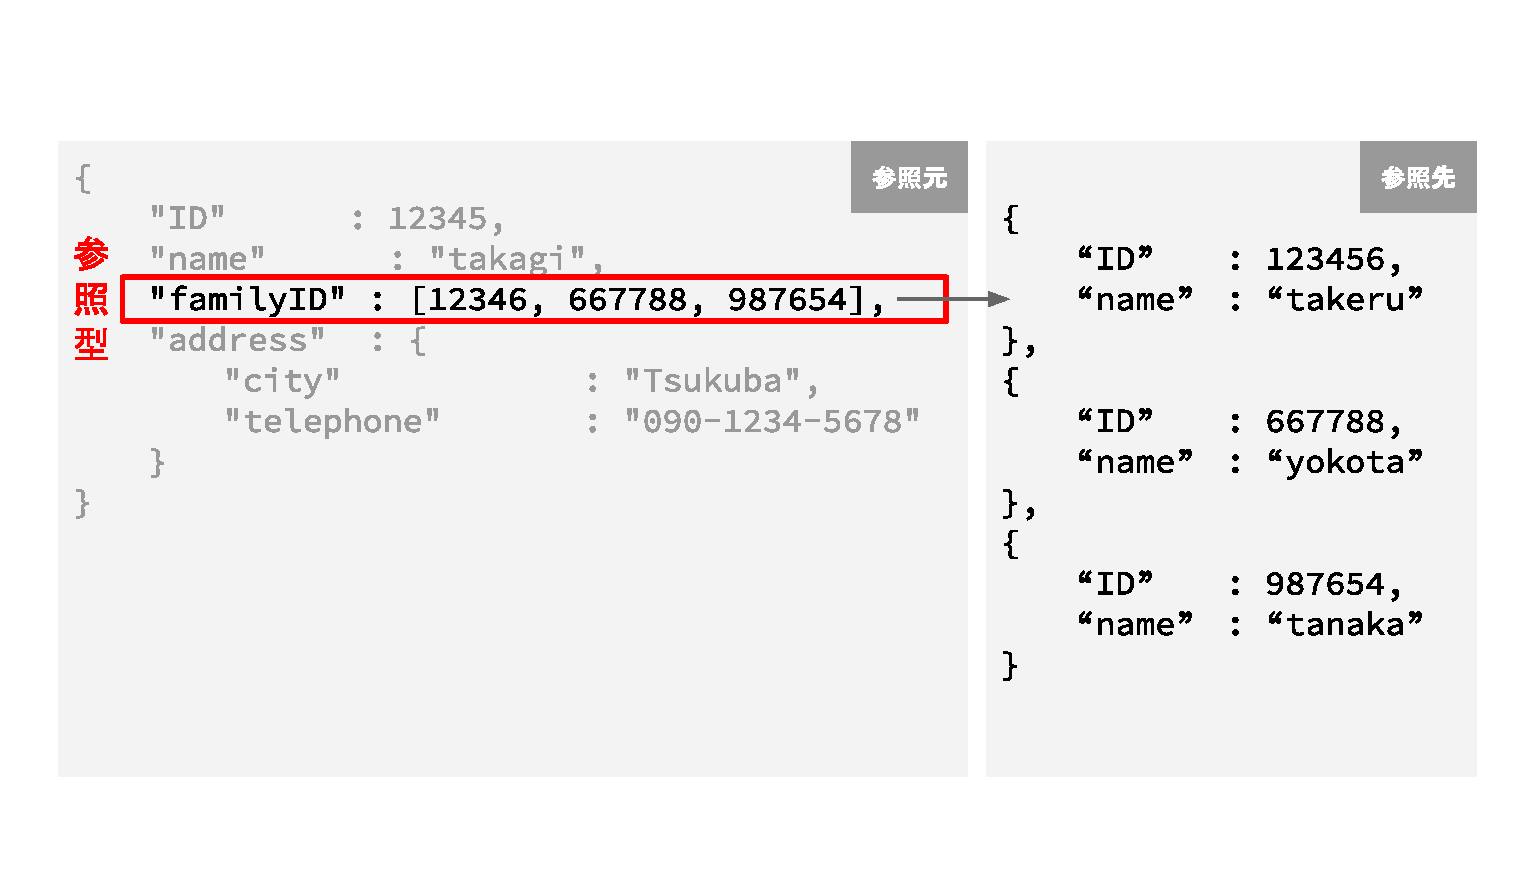
\includegraphics[width=30em, trim=0 5em 0 2em]{/Users/takagihayata/workspace/materialize-mongodb/paper/mast/src/Reference.eps} %[trim=left bottom right top]
	\end{center}
	\caption{参照型}
	\label{figure:Reference}
\end{figure}
\begin{figure}[htbp]
	\begin{center}
		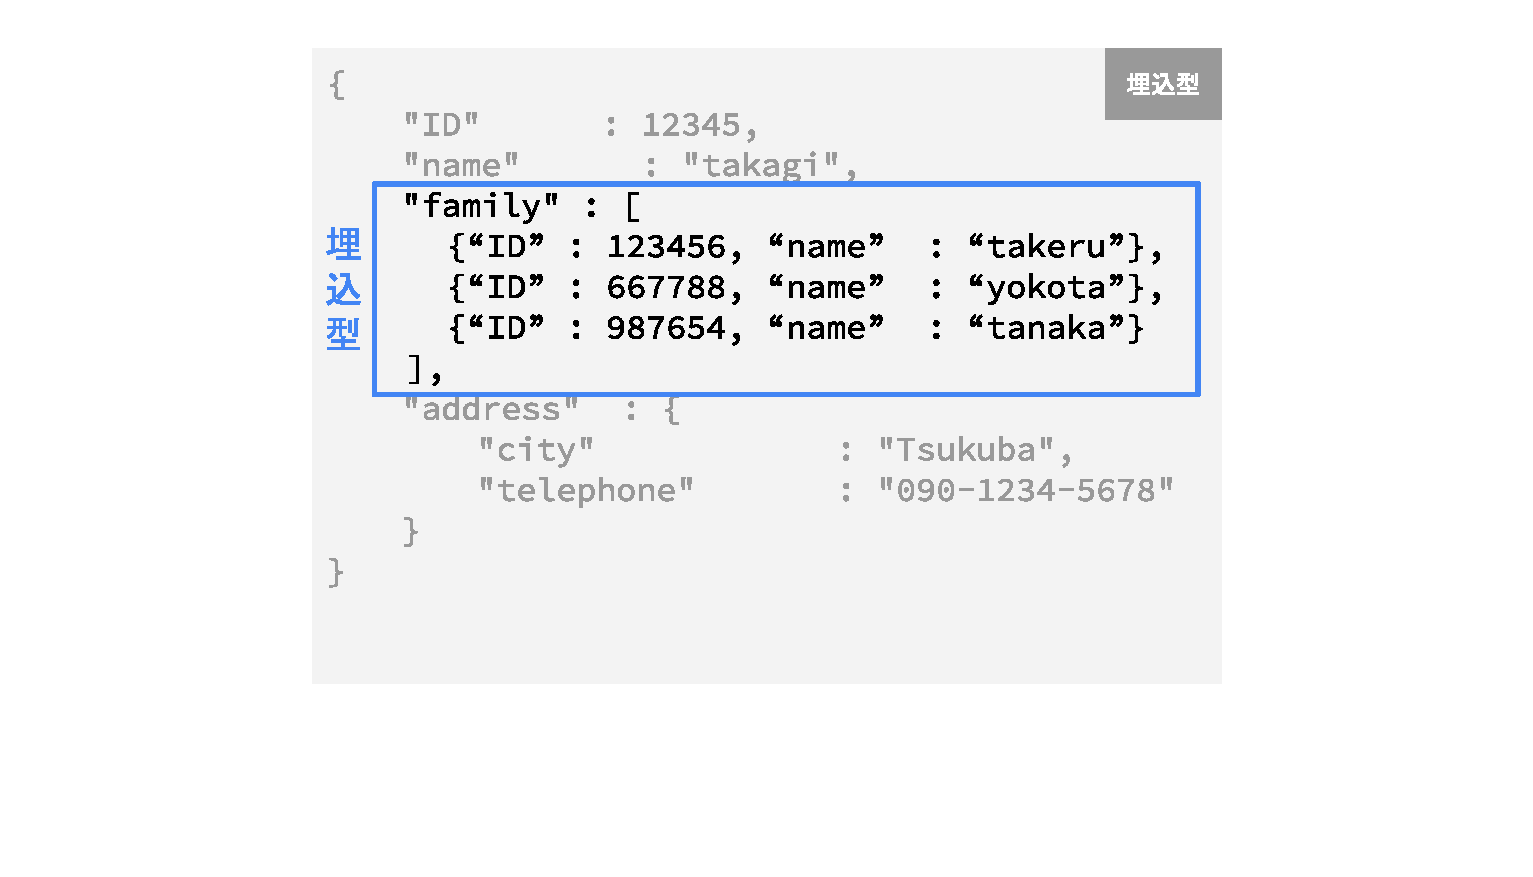
\includegraphics[width=30em, trim=0 7em 0 0em]{/Users/takagihayata/workspace/materialize-mongodb/paper/mast/src/Embed.eps} %[trim=left bottom right top]
	\end{center}
	\caption{埋込型}
	\label{figure:Embed}
\end{figure}

\begin{table}[htb]
  \begin{center}
    \caption{MongoDBにおける参照型データモデルと埋込型データモデルでの検索クエリ}
		\label{table:MongoReferenceEmbedFind}
    \begin{tabular}{|c|l|} \hline
			参照型 &
			\begin{tabular}{l}
				db.people.aggregate([\{ \$match: \{ID: 12345\}\},\\ \{ \$lookup: \{ from: "families", localField: "familyID", foreignField: "ID"\}\}]);
			\end{tabular}\\ \hline
			埋込型 &
			\begin{tabular}{l}
				db.people.find(\{ID: 12345\});
			\end{tabular}
			  \\ \hline
    \end{tabular}
  \end{center}
\end{table}
\begin{table}[htb]
  \begin{center}
    \caption{MongoDBにおける参照型データモデルと埋込型データモデルでの更新クエリ}
		\label{table:MongoReferenceEmbedUpdate}
    \begin{tabular}{|c|l|} \hline
			参照型 &
			\begin{tabular}{l}
				db.family.update(\{ ID: 123456\},\{ \$set: \{ name: "takebayashi"\}\});
			\end{tabular}\\ \hline
			埋込型 &
			\begin{tabular}{l}
				db.people.update(\{"family.ID": 12345\}, \{ \$set: \{family.\$.name: "takebayashi"\}\});
			\end{tabular}
			  \\ \hline
    \end{tabular}
  \end{center}
\end{table}

全てのドキュメントを埋め込み型として保存すると埋め込み先のドキュメントの更新処理が増え,著しく更新時間が増加する為,データモデルとして最適とは言えない.埋め込み型のデータモデルとして保存するコレクションを最適に選択し,データモデルを最適化することがドキュメント指向型データベースを高速に使用することに繋がる.本論文ではこの実体化するコレクションの選択を自動化する.

\section{提案手法の構成}
本論文ではドキュメント指向型データベースの埋込型データモデルをリレーショナルデータベースの実体化ビューと置き換えて考える.ドキュメント指向型データベースのよくアクセスされる部分や処理速度がネックとなっている部分を埋込型として別コレクションに保持することで“実体化ビュー作成”,どの部分を埋込型にするかの判断を“実体化ビュー選択”とする.図\ref{figure:ReferenceToEmbed}は本論文での“実体化ビュー作成”を示したものである.
\begin{figure}[htbp]
	\begin{center}
		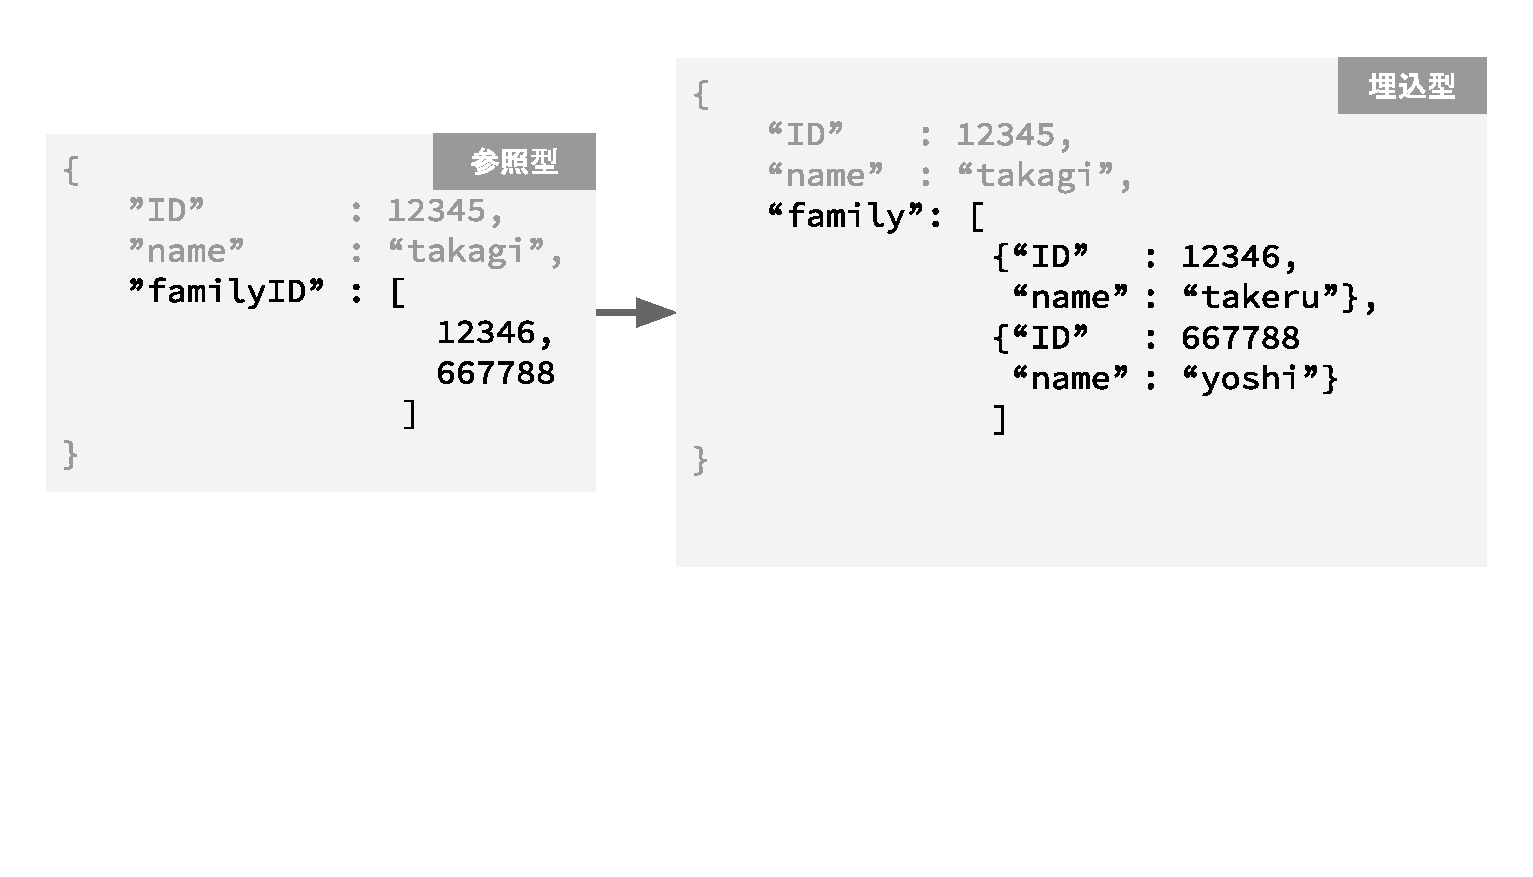
\includegraphics[width=30em, trim=0 13em 0 0]{/Users/takagihayata/workspace/materialize-mongodb/paper/mast/src/ReferenceToEmbed.eps} %[trim=left bottom right top]
	\end{center}
	\caption{参照型から埋込型への書き換え}
	\label{figure:ReferenceToEmbed}
\end{figure}

実装システムについて図\ref{figure:Midleware}に示す.ユーザーからのデータアクセスから実体化ビュー作成までの流れを図\ref{figure:Midleware}を用いて説明する.
\begin{figure}[h]
	\begin{center}
		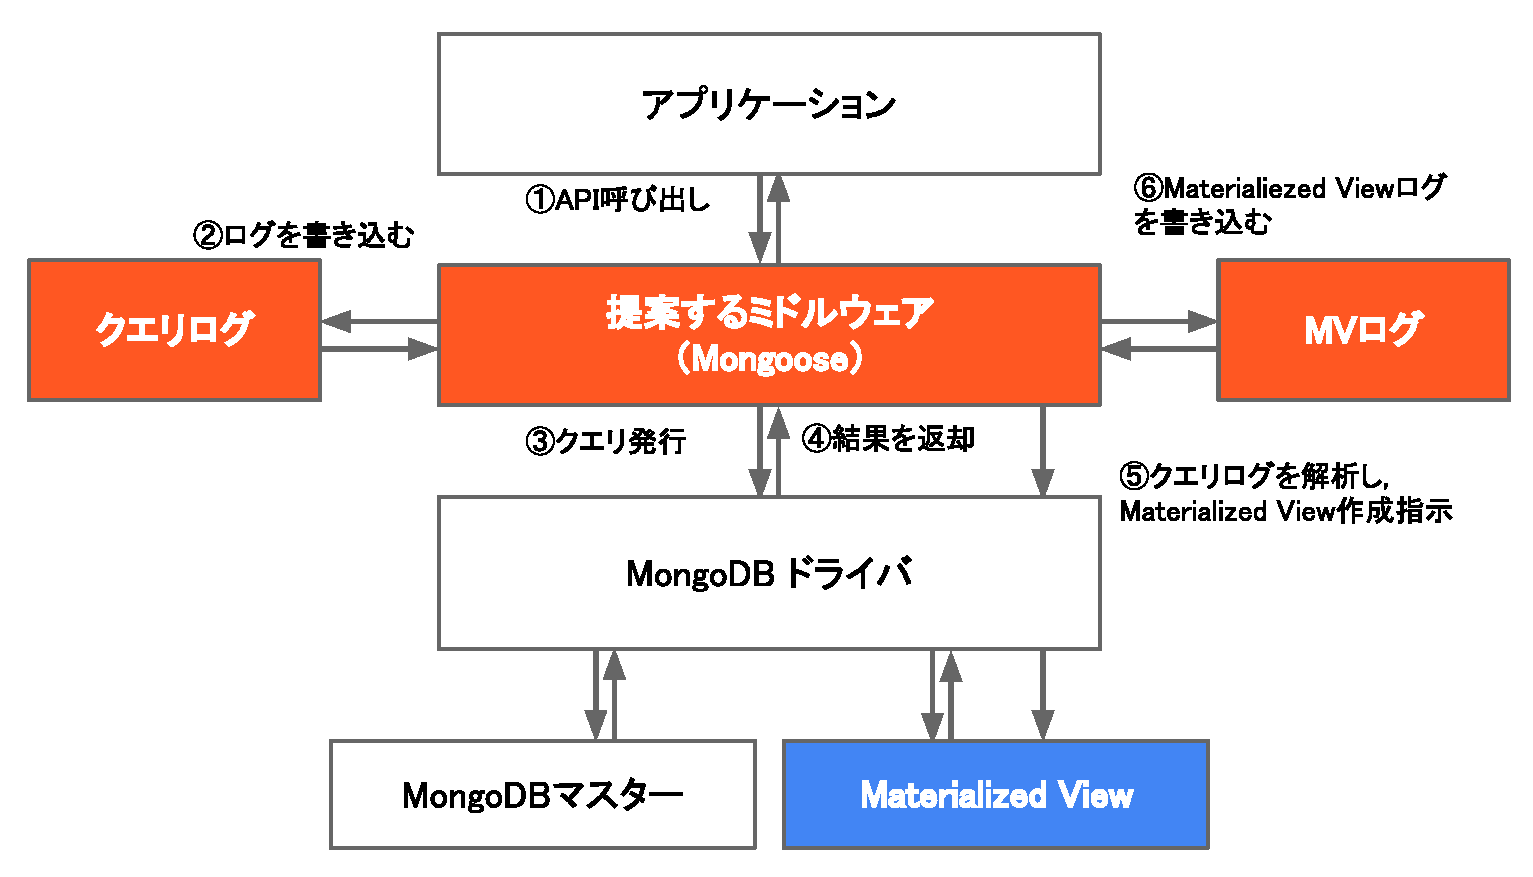
\includegraphics[width=30em]{/Users/takagihayata/workspace/materialize-mongodb/paper/mast/src/Midleware.eps}
	\end{center}
	\caption{提案ミドルウェア(実体化前)}
	\label{figure:Midleware}
\end{figure}
図\ref{figure:Midleware}-①まずユーザーがアプリケーションからミドルウェアに対してデータアクセスの要求する.図\ref{figure:Midleware}-②ミドルウェアでは,頻繁にアクセスされるドキュメントを分析するために,クエリに関するログを残す.図\ref{figure:Midleware}-③次にMongoDBに対してクエリを発行する.図\ref{figure:Midleware}-④MongoDBから返ってきたクエリセットをアプリケーションに返却する.図\ref{figure:Midleware}-⑤クエリログを解析し,ボトルネックとなっているところや呼び出し回数の多い条件の実体化ビューを作成する.図\ref{figure:Midleware}-⑥実体化したドキュメントに関してログに記録する.

実体化した後のデータアクセスの流れを図\ref{figure:MidlewareMv}に示す.図\ref{figure:MidlewareMv}-①’アプリケーションからデータベースにアクセスがあった場合,まずログからアクセスされたデータが実体化されているか判定する.図\ref{figure:MidlewareMv}-②’実体化されている場合はクエリを書き換えて実体化ビューから結果を取得する.図\ref{figure:MidlewareMv}-③’アプリケーションに結果を返す際には元のクエリに合うように適宜変換する.
\begin{figure}[htbp]
	\begin{center}
		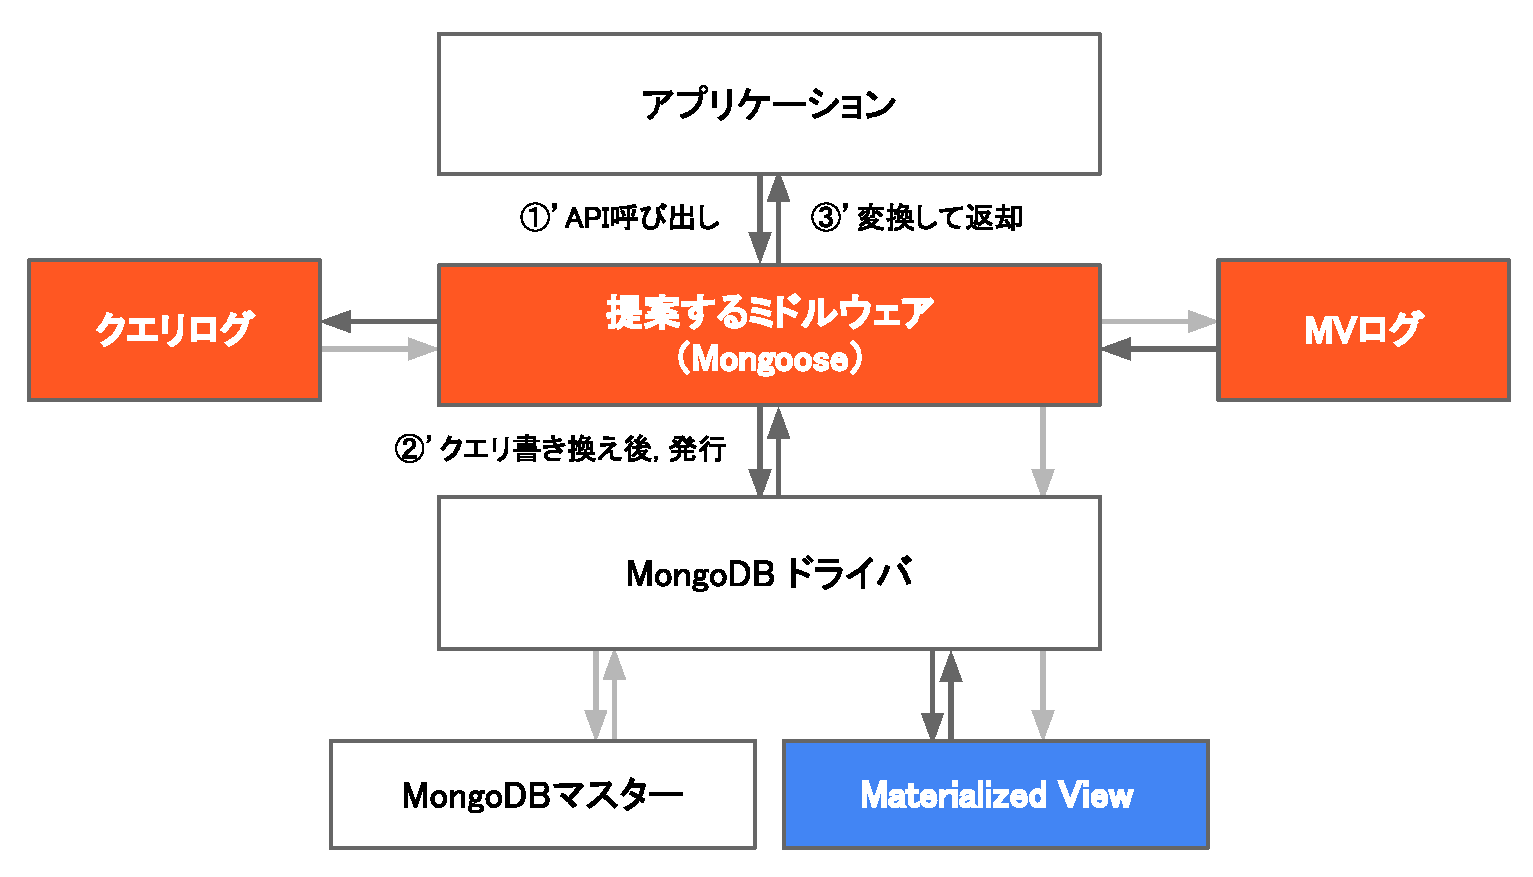
\includegraphics[width=30em]{/Users/takagihayata/workspace/materialize-mongodb/paper/mast/src/MidlewareMv.eps} %[trim=left bottom right top]
	\end{center}
	\caption{提案ミドルウェア(実体化後)}
	\label{figure:MidlewareMv}
\end{figure}

\section{実体化アルゴリズムについて}
クエリログから実体化するコレクションを決定する条件を適切に設定することで,実体化ビュー選択を自動化することができる.この実体化条件については以下の条件が考えられる.
\begin{enumerate}
  \item クエリログの統計
  \item ドキュメント内の参照数
\end{enumerate}
1の条件は実際のクエリの検索回数・更新回数やその処理時間を元に実体化するコレクションを選定する.2の条件ではドキュメント内の他コレクションへの参照数を元に実体化後の更新処理の増加を予想し,実体化するコレクションを選定する.本論文では更新処理が用意であり,クエリに柔軟に対応できるクエリログの統計を元に実体化する条件を作成する.

\section{逆実体化アルゴリズムについて}
クエリのログを元に実体化した場合,クエリの傾向が変わることで実体化していない状態の方が望ましくなる可能性や,コレクションの特性によっては実体化によるメリットがデメリットより少ない可能性がある.そのような事を防ぐために,定期的に実体化したコレクションに対してもメンテナンスを行い,場合によっては実体化したコレクションをオリジナルのデータモデルに戻すことが必要である.本論文では実体化したコレクションのデータモデルを元に戻す事を逆実体化と定義する.この逆実体化に対しても実体化同様,適切な逆実体化条件を設定する必要がある.

本論文ではクエリのログの統計から実体化後の検索処理時間と更新処理時間を比較し,各コレクションに対して逆実体化の必要性を確認する.

\end{document}
